%=========================================================================
% (c) 2011, 2012 Josef Lusticky

\section{Kernel and processes}\label{sec:contiki-kernel}
The kernel in Contiki is event-driven and provides a cooperative multitasking
environment, but the system supports preemptive
multithreading that can be applied on a per-process basis~\cite{video}.
The preemption is not implemented in the kernel, but
preemptive multithreading is implemented as a library that is linked only with programs that
explicitly require multithreading~\cite{paper-contiki}.
The kernel itself contains no platform specific code, it implements only CPU multiplexing and
lets device drivers and applications communicate directly with hardware~\cite{video}.

From high levels of abstraction,
applications in Contiki OS are implemented and run as processes.
Protothreads, the lightweight threads described in section~\ref{sec:contiki-protothreads},
are used in Contiki to implement processes.
Both the Contiki kernel and Contiki applications use
Protothreads extensively to achieve cooperative multitasking~\cite{contiki-wiki-faq}.
Every Contiki process consists of a process control block and a process thread~\cite{contiki-wiki-processes}.
The process control block contains run-time information about the process and
the process thread contains the code of the process.
Among other things, the process control block contains
the textual name of the process, a pointer to the process thread and state of the process.
The process thread is implemented as a single Protothread,
that is invoked from the process scheduler in the Contiki kernel~\cite{contiki-wiki-processes}.

From low levels of abstraction,
every application is implemented as a simple C function
and the process control block remembers the actual state of execution of this function
in the same way as the local continuation works by Protothreads.
Processes are therefore running quasi-parallel in Contiki.

The process control block is not declared or defined directly,
but through the {\it{PROCESS()}} macro.
This macro takes two parameters: the variable name of the process control block
and a textual name of the process,
which is used in debugging and when printing out lists of active processes to users~\cite{contiki-wiki-processes}.
The process control block is shown in listing~\ref{lst:contiki-pcb}.
\bigskip
\begin{lstlisting}[caption={Process control block in Contiki OS},label={lst:contiki-pcb}]
struct process {
	struct process *next;
	const char *name;
	int (* thread)(struct pt *, process_event_t, process_data_t);
	struct pt pt;
	unsigned char state, needspoll;
	};
\end{lstlisting}

All code execution is initiated by the Contiki kernel
that acts like a simple dispatcher calling these functions~\cite{contiki-docs}.
Just like Protothreads, processes are also implemented using macros,
making them fully standard C compatible.

In Contiki, code runs in either of two execution contexts:
cooperative, in which code never preempts other code, and preemptive,
which preempts the execution of cooperative code and returns control
when preemptive code is finished.
Processes always run in cooperative mode,
whereas interrupt service routines and real-time timers run in preemptive mode~\cite{contiki-wiki-processes}.
Code running in both execution contexts illustrates figure~\ref{fig:contiki-execution-context}.

\begin{figure}
  \centering
  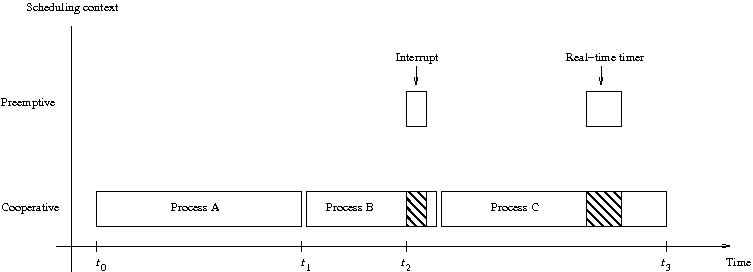
\includegraphics[width=13cm,keepaspectratio]{fig/Execution-contexts.png}
  \caption{Contiki execution contexts (source:~\cite{contiki-wiki-processes})}
  \label{fig:contiki-execution-context}
\end{figure}

Interprocess communication is done by posting events in Contiki OS -
processes communicate with each other by posting events to each other~\cite{paper-contiki}.
There are two types of events: synchronous and asynchronous.
Synchronous events are directly delivered to the receiving process when posted and
can only be posted to a specific processes~\cite{contiki-wiki-processes}.
Because synchronous events are delivered immediately,
posting synchronous event is equivalent to a function call:
the process to which an event is delivered is directly invoked,
and the process that posted the event is blocked
until the receiving process has finished processing the event~\cite{contiki-wiki-processes}.

Asynchronous events are delivered to the receiving process
some time after they have been posted~\cite{contiki-wiki-processes}.
Before delivery, the asynchronous events are held on an event queue inside the Contiki kernel.
The kernel loops through this event queue and delivers
the event to the process by invoking the process.
The receiver of an asynchronous event can be either a specific process
or all running processes~\cite{contiki-wiki-processes}.

%! paper-contiki - dunkels04contiki
%Being able to power down the device
%when the network is inactive is often required way to reduce energy consumption.
%Power conservation mechanisms
%depend on both the applications and the network protocols.
%The Contiki kernel contains no explicit power
%save abstractions, but lets the the application specific parts
%of the system implement such mechanisms.
%To help the application decide when to power down the system, the event
%scheduler exposes the size of the event queue.
%This information can be used to power down the processor when there
%are no events scheduled.
%! paper-contiki

%As stated before, Contiki is well documented and you can find out more about
%the kernel as well as the system in the documentation~\cite{contiki-docs}.
